Trong mối quan hệ bất đối xứng, một bối cảnh bị giới hạn có sự phụ thuộc vào một bối cảnh bị giới hạn khác. Mối quan hệ này được mô tả bằng cách gán vai trò cho bối cảnh bị giới hạn :

\begin{itemize}

\item \textbf{Bối cảnh bị giới hạn thượng nguồn (Upstream):}

\begin{itemize}

\item Bối cảnh bị giới hạn cung cấp cho bối cảnh bị giới hạn khác.

\item Ký hiệu: U

\end{itemize}

\item \textbf{Bối cảnh bị giới hạn hạ lưu (Downstream):}

\begin{itemize}

\item Bối cảnh bị giới hạn phụ thuộc vào bối cảnh bị giới hạn khác.

\item Ký hiệu: D

\end{itemize}

\end{itemize}

\begin{example} Mối quan hệ bất đối xứng giữa bối cảnh bị giới hạn A và bối cảnh bị giới hạn B.

\begin{itemize}

\item Bối cảnh bị giới hạn A ràng buộc với bối cảnh bị giới hạn B

\item Bối cảnh bị giới hạn A đóng vai trò là bối cảnh bị giới hạn hạ lưu (Downstream)

\item Bối cảnh bị giới hạn B đóng vai trò là bối cảnh bị giới hạn thượng nguồn (Upstream)

\item Bối cảnh bị giới hạn A có kiến thức về các mô hình trong bối cảnh bị giới hạn B

\item Bối cảnh bị giới hạn B không có bất kỳ kiến thức nào về mô hình trong bối cảnh bị giới hạn A

\end{itemize}

\begin{figure}[H]

\centering

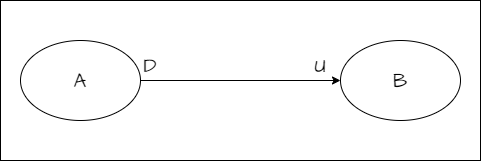
\includegraphics[scale = 0.5]{pictures/moi_quan_he_bat_doi_xung/main.drawio.png}

\caption{Ví dụ mối quan hệ bất đối xứng}

\end{figure}

\end{example}